\documentclass[aspectratio=169]{beamer}
\usetheme{Madrid}
\usecolortheme{dolphin}
\usepackage{tikz}
\usepackage{amsmath, amssymb}
\usepackage{graphicx}
\usepackage{hyperref}
\usepackage[utf8]{vietnam}
\title{Cây Khung và Lowest Common Ancestor (LCA)}
\author{Nhóm 7}
\date{\today}

\begin{document}

\frame{\titlepage}

\begin{frame}{Nội dung}
\tableofcontents
\end{frame}

\section{Giới thiệu Cây Khung}
\begin{frame}{Định nghĩa Cây Khung}
\begin{itemize}
    \item \textbf{Đồ thị vô hướng có trọng số dương} $G=(V,E)$
    \item \textbf{Cây khung} (Spanning Tree - ST): tập con $T\subseteq E$ nối tất cả các đỉnh mà không tạo chu trình.
    \item \textbf{Minimum Spanning Tree (MST)}: ST có tổng trọng số nhỏ nhất.
\end{itemize}
\end{frame}

\begin{frame}{Bài toán MST}
\textbf{Input:} đồ thị $G=(V,E)$ với trọng số $w(e)$ cho mỗi cạnh.

\textbf{Output:} tập cạnh $T$ sao cho:
\begin{itemize}
    \item $T$ tạo cây khung
    \item Tổng trọng số $\sum_{e\in T} w(e)$ là nhỏ nhất
\end{itemize}
\end{frame}

\begin{frame}{Thuật toán Kruskal}
\begin{enumerate}
    \item Sắp xếp tất cả các cạnh theo trọng số tăng dần
    \item Lấy cạnh nhỏ nhất, thêm vào MST nếu không tạo chu trình
    \item Dùng \textbf{Union-Find} để kiểm tra chu trình
    \item Lặp lại đến khi có $|V|-1$ cạnh
\end{enumerate}
\end{frame}

\begin{frame}{Thuật toán Prim}
\begin{enumerate}
    \item Chọn đỉnh bắt đầu
    \item Thêm cạnh nhỏ nhất nối đỉnh trong MST với đỉnh ngoài MST
    \item Lặp lại đến khi tất cả đỉnh được nối
\end{enumerate}
\end{frame}

\begin{frame}{Ví dụ MST}
\begin{center}
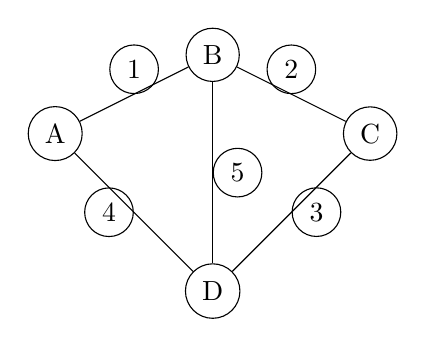
\begin{tikzpicture}[scale=1, every node/.style={circle,draw}]
\node (A) at (0,0) {A};
\node (B) at (2,1) {B};
\node (C) at (4,0) {C};
\node (D) at (2,-2) {D};
\draw (A) -- node[above]{1} (B);
\draw (B) -- node[above]{2} (C);
\draw (C) -- node[right]{3} (D);
\draw (A) -- node[left]{4} (D);
\draw (B) -- node[right]{5} (D);
\end{tikzpicture}

MST gồm các cạnh có trọng số 1,2,3.
\end{center}
\end{frame}

\section{Giới thiệu LCA}
\begin{frame}{Định nghĩa LCA}
\begin{itemize}
    \item Cho cây gốc $T$ và hai đỉnh $u,v$
    \item \textbf{Lowest Common Ancestor (LCA)} của $u$ và $v$ là đỉnh sâu nhất $w$ sao cho $w$ là tổ tiên của cả $u$ và $v$
\end{itemize}
\end{frame}

\begin{frame}{Bài toán LCA}
\textbf{Input:} Cây $T$ và nhiều truy vấn $(u,v)$

\textbf{Output:} LCA(u,v) cho mỗi truy vấn

\textbf{Ứng dụng:} khoảng cách giữa hai đỉnh, kiểm tra thuộc cây, DP trên cây
\end{frame}

\begin{frame}{Ý tưởng thuật toán LCA - Binary Lifting}
\begin{itemize}
    \item Tiền xử lý $2^k$ tổ tiên của mỗi đỉnh
    \item Tìm LCA(u,v) bằng cách nâng u,v lên cùng độ sâu và nhảy theo lũy thừa của 2
    \item Thời gian: $O(N\log N)$ tiền xử lý, $O(\log N)$ truy vấn
\end{itemize}
\end{frame}

\begin{frame}{Cấu trúc dữ liệu Binary Lifting}
\begin{itemize}
    \item $up[v][k]$ = tổ tiên thứ $2^k$ của $v$
    \item $depth[v]$ = độ sâu của $v$ so với gốc
    \item Khởi tạo DFS:
    \begin{itemize}
        \item up[v][0] = parent[v]
        \item up[v][k] = up[up[v][k-1]][k-1]
    \end{itemize}
\end{itemize}
\end{frame}

\begin{frame}{Thuật toán truy vấn LCA}
\begin{enumerate}
    \item Nếu $depth[u]<depth[v]$, đổi chỗ u,v
    \item Nâng u lên cùng độ sâu với v
    \item Nâng đồng thời u và v theo lũy thừa 2 đến khi up[u][0]=up[v][0]
    \item Trả về tổ tiên chung
\end{enumerate}
\end{frame}

\begin{frame}{Ví dụ minh họa LCA}
\begin{center}
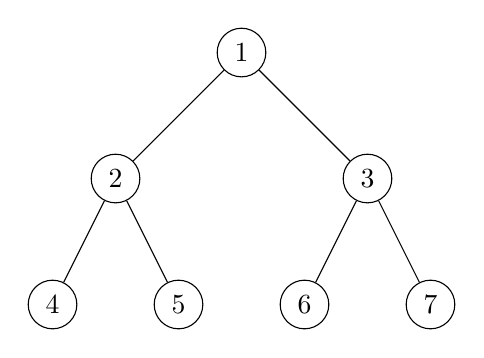
\begin{tikzpicture}[scale=0.8, every node/.style={circle,draw}]
\node (1) at (0,0) {1};
\node (2) at (-2,-2) {2};
\node (3) at (2,-2) {3};
\node (4) at (-3,-4) {4};
\node (5) at (-1,-4) {5};
\node (6) at (1,-4) {6};
\node (7) at (3,-4) {7};
\draw (1) -- (2);
\draw (1) -- (3);
\draw (2) -- (4);
\draw (2) -- (5);
\draw (3) -- (6);
\draw (3) -- (7);
\end{tikzpicture}

LCA(4,5)=2, LCA(4,6)=1
\end{center}
\end{frame}

\section{Mô phỏng thuật toán}
\begin{frame}{Mô phỏng MST và LCA}
\begin{itemize}
    \item Bước 1: Xây MST từ đồ thị
    \item Bước 2: Chọn gốc cây, DFS để tính depth và up[][]
    \item Bước 3: Xử lý truy vấn LCA
\end{itemize}
\end{frame}

\begin{frame}{Ví dụ bài tập}
\textbf{Bài tập:} Cho đồ thị: 
\begin{itemize}
    \item 5 đỉnh, 7 cạnh
    \item Tìm MST
    \item Chọn đỉnh 1 làm gốc, tìm LCA(4,5)
\end{itemize}
\end{frame}

\begin{frame}{Giải bài tập ví dụ}
\begin{itemize}
    \item MST gồm các cạnh có trọng số nhỏ nhất nối tất cả đỉnh
    \item Dùng DFS tính depth, up[][]
    \item LCA(4,5)=...? Từ mô phỏng trên cây
\end{itemize}
\end{frame}

\begin{frame}{Tổng kết}
\begin{itemize}
    \item MST: cây nối tất cả đỉnh với tổng trọng số nhỏ nhất
    \item LCA: tìm tổ tiên chung thấp nhất giữa hai đỉnh
    \item Thuật toán Binary Lifting: tối ưu truy vấn LCA
    \item Ứng dụng: đường đi ngắn nhất trong cây, DP, kiểm tra quan hệ tổ tiên
\end{itemize}
\end{frame}

\begin{frame}{Tài liệu tham khảo}
\begin{itemize}
    \item Cormen, Leiserson, Rivest, Stein: Introduction to Algorithms
    \item Competitive Programming 3 - Steven Halim
    \item CP-Algorithms: https://cp-algorithms.com/graph/lca.html
\end{itemize}
\end{frame}

\end{document}